\documentclass[a4paper,12pt]{article}
\usepackage[margin=1in]{geometry}

\usepackage[T2A]{fontenc}			% кодировка
\usepackage[utf8]{inputenc}			% кодировка исходного текста
\usepackage[english,russian]{babel}	% локализация и переносы
\usepackage{graphicx}                % Математика
\usepackage{amsmath,amsfonts,amssymb,amsthm,mathtools} 
\usepackage{mathtext}
\usepackage[T2A]{fontenc}
\usepackage[utf8]{inputenc}

\usepackage{wasysym}

%Заговолок
\author{Бичина Марина 
группа Б04-005 1 курса ФЭФМ}
\title{}
\date{}


\begin{document} % начало документа

\begin{center}
\begin{Large}
{ Марина Б04-005, Лабораторная работа №.3.4.1:
Диа- и парамагнетики}
\end{Large}
\end{center}
\paragraph{Цель работы:} 
\begin{enumerate}
\itemsep0em
\item Исследовать зависимость силы, действующей на образец, размещенный в зазоре электромагнита, от величины поля в зазоре 
\item Рассчитать магнитную восприимчивость меди и алюминия
\end{enumerate}
\paragraph{Оборудование:}
\begin{enumerate}
\itemsep0em
\item электромагнит
\item аналитические весы
\item милливеберметр
\item регулируемый источник постоянного тока
\item образцы
\end{enumerate}


\paragraph{Теоретическая справка:}
\paragraph{Магнитная восприимчивость} тела может быть определена измерением сил, действующих на это тело в магнитном поле. Существуют два классических метода таких измерений: метод \textit{Фарадея }и метод \textit{Гюи}. В методе Гюи используется тонкий и длинный стержень, один из концов которого помещают в зазор электромагнита (в область однородного поля), а другой конец -- вне зазора, где величиной магнитного поля можно пренебречь. Тогда сила, действующая на помещённый образец равна:

\[
F_m = \left( \frac{\partial W_m}{\partial x} \right) \approx \chi \frac{B_0^2}{2 \mu_0} S.
\]

Знак силы зависит от восприимчивости $\chi$: парамагнетики $(\chi > 0)$ втягиваются в зазор электромагнита, а диамагнетики $(\chi < 0)$ выталкиваются из него. Таким образов рассчитав силу действующую на образец в известном магнитном поле, можно рассчитать его магнитную восприимчивость.


\paragraph{Описание установки:}
\paragraph{}
Схема установки приведена на рис. \ref{fig:setup}.

 Она состоит из:
\begin{enumerate}
\itemsep0em
\item Электромагнита с зазором. Поле в зазоре можно считать практически однородным
так как размеры полюсов значительно превышают размер зазора. 
\item Источника питания с регулируемым постоянным током. Величина тока задаётся при
помощи амперметра. Дли градуировки электромагнита используется \item милливеберметрa.
\item Весов на которые подвешивается образец.
\end{enumerate}
\begin{figure}
\begin{center}
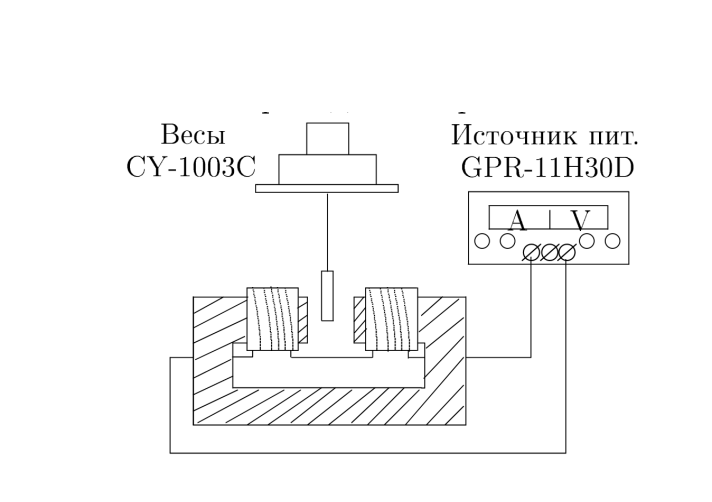
\includegraphics[width=0.5\linewidth]{setup.png}
\caption{Схема экспериментальной установки}
\label{fig:setup}
\end{center}
\end{figure}

\paragraph{Ход работы:}
\begin{enumerate}
\itemsep0em
\item Измерим индукцию магнитного поля в зазоре милливеберметром, пользуясь 
формулой $B = \Phi / S_n$. Значение $S_n = 72$ см$^2$. Измерим поток $\Phi$ между полюсами
при различных значениях тока на обмотке электромагнита, и посчитаем индукцию. Результаты измерений предствалены в таблице \ref{tab:grad}, на основании который построен график \ref{fig:grad_plot}. Погрешность измерения силы тока $\Delta I = 0.01$ А, погрешность милливеберметра $\Delta \Phi = 0.05$ мВб, и следовательно погрешность измерения $\Delta B = \Delta \Phi / S_n = 7$ мТл.

\begin{table}[h]
\begin{center}
\begin{tabular}{|c|c|c|c|c|c|c|c|c|}
\hline 
$I$, А & 0.3 & 0.7 & 1.1 & 1.5 & 1.9 & 2.3 & 2.6 & 3.0 \\ 
\hline 
$\Phi$, мВб & 0.4 & 1.3 & 2.7 & 3.6 & 4.5 & 5.4 & 6 & 6.7 \\ 
\hline 
$B$, мТл & 56 & 181 & 375 & 500 & 625 & 750 & 833 & 931 \\ 
\hline 
\end{tabular}
\caption{Данные для градуировки электромагнита} 
\label{tab:grad}
\end{center}
\end{table}

\begin{figure}[h!]
\begin{center}
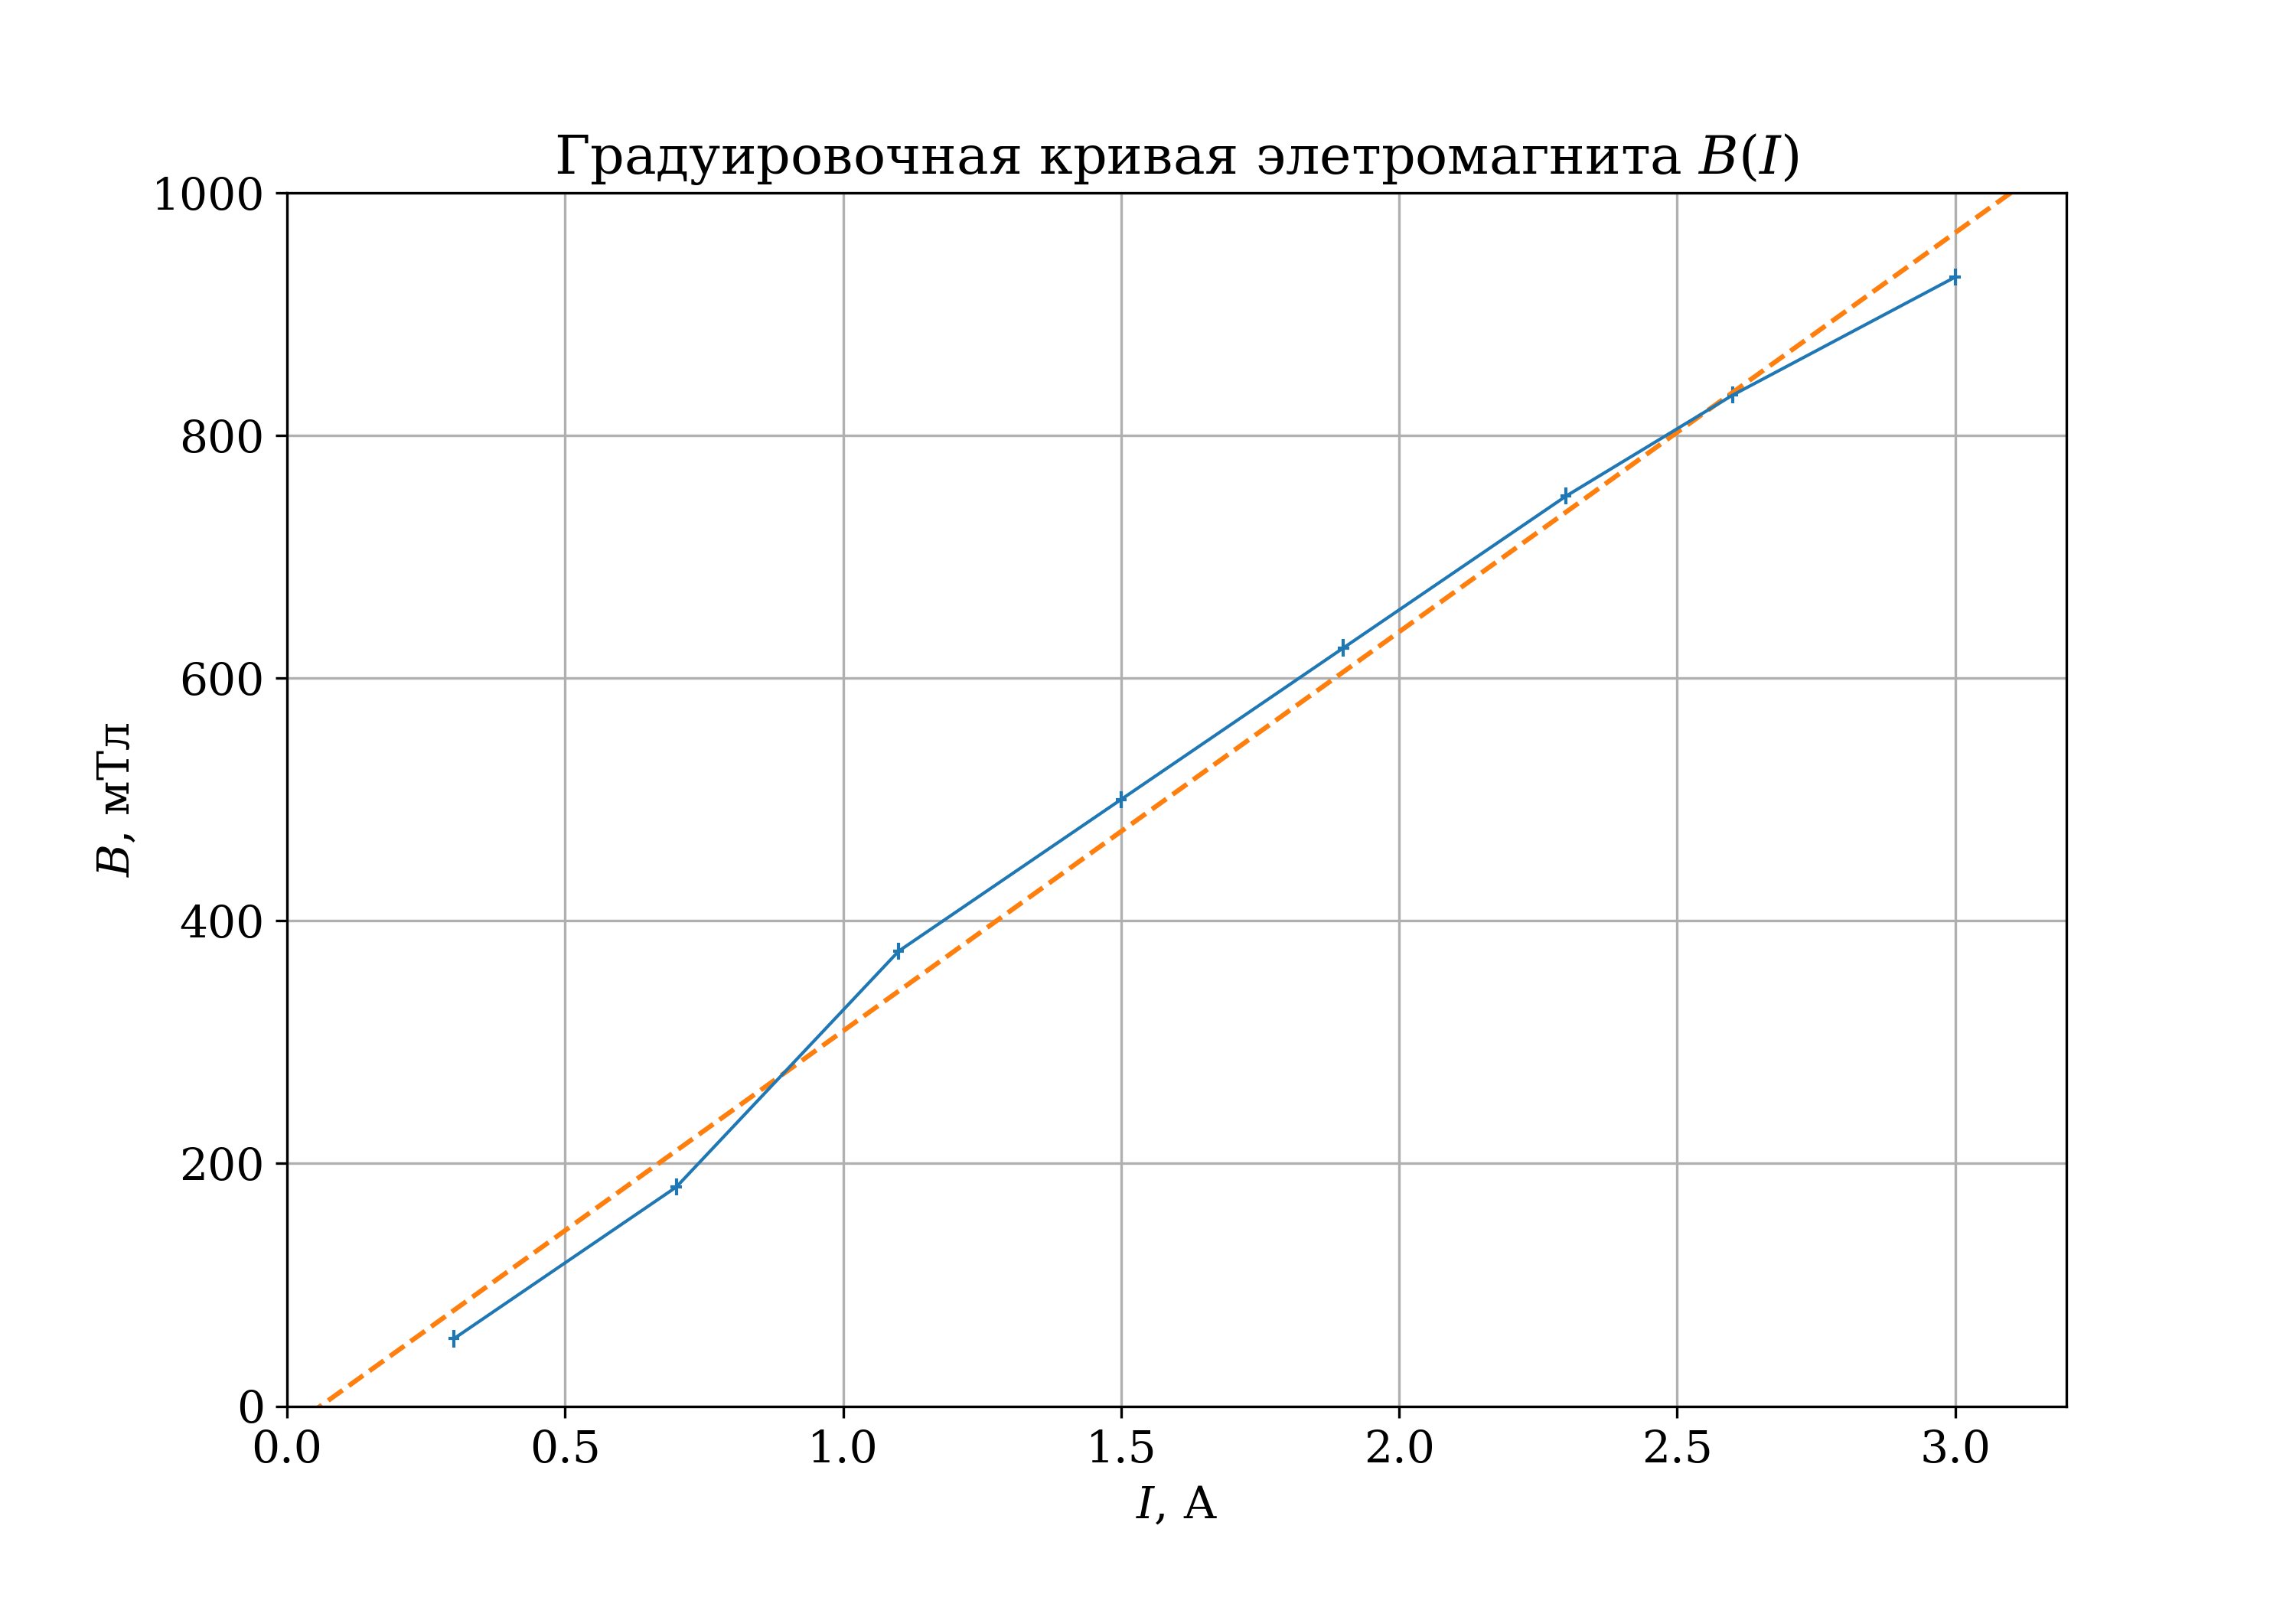
\includegraphics[width=0.85\linewidth]{grad_plot.png}
\caption{График градуировочной кривой}
\label{fig:grad_plot}
\end{center}
\end{figure}


\item  Измерим перегрузку $\Delta P$ для образцов при различных значениях тока. Для этого снимем показания весов $\Delta M$ при различных значениях $I$ и домножим на коэффициент $g$ ($P = mg$). Данные занесём в таблицу \ref{tab:measure}, значения снятые при увеличении и уменьшении силы тока помечены значками $\blacktriangle$ и $\blacktriangledown$ соответственно.

\begin{table}[h]
\begin{center}
\begin{tabular}{|c||c|c|c|c|c|c|c|c|c|}
\hline 
$I$ & 0 & 0.3 & 0.7 & 1.1 & 1.5 & 1.9 & 2.3 & 2.6 & 3.0 \\ 
\hline 
$\Delta M \blacktriangle$ Cu, мг & 0 & 0 & -2 & -4 & -6 & -11 & -14 & -17 & -21 \\ 
\hline 
$\Delta M \blacktriangledown$ Cu, мг & 0 & -2 & -3 & -6 & -9 & -12 & -16 & -18 & -- \\ 
\hline 
$\Delta P \blacktriangle$ Cu, мкН & 0 & 0 & -20 & -39 & -59 & -108 & -137 & -166 & -206 \\ 
\hline 
$\Delta P \blacktriangledown$ Cu, мкН & 0 & -20 & -30 & -59 & -88 & -118 & -157 & -176 & -- \\ 
\hline 
$\Delta M \blacktriangle$ Al, мг & 0 & 0 & 1 & 4 & 10 & 17 & 26 & 32 & 41 \\ 
\hline 
$\Delta M \blacktriangledown$ Al, мг & 2 & 2 & 2 & 7 & 11 & 19 & 27 & 34 & -- \\ 
\hline 
$\Delta P \blacktriangle$ Al, мкН & 0 & 0 & 10 & 39 & 98 & 166 & 255 & 314 & 402 \\ 
\hline 
$\Delta P \blacktriangledown$ Al, мкН & 20 & 20 & 20 & 69 & 108 & 186 & 265 & 333 & -- \\ 
\hline 
$\Delta M \blacktriangle$ C, мг & 0 & 8 & 24 & 37 & 39 & 39 & 34 & 28 & 10 \\ 
\hline 
$\Delta M \blacktriangledown$ C, мг & 8 & 17 & 33 & 46 & 46 & 46 & 37 & 26 & -- \\ 
\hline 
$\Delta P \blacktriangle$ C, мкН & 0 & 78 & 235 & 363 & 382 & 382 & 333 & 274 & 98 \\ 
\hline 
$\Delta P \blacktriangledown$ C, мкН & 78 & 167 & 323 & 451 & 451 & 451 & 363 & 255 & -- \\ 
\hline 
\end{tabular} 
\caption{Снятые экспериментальные данные}
\label{tab:measure}
\end{center}
\end{table}

\item Отметим измеренные значения на графике и проведём аппроксимирующие кривые (рис. \ref{plot_cu}, \ref{plot_al}, \ref{plot_c}).

\begin{figure}[h!]
\begin{center}
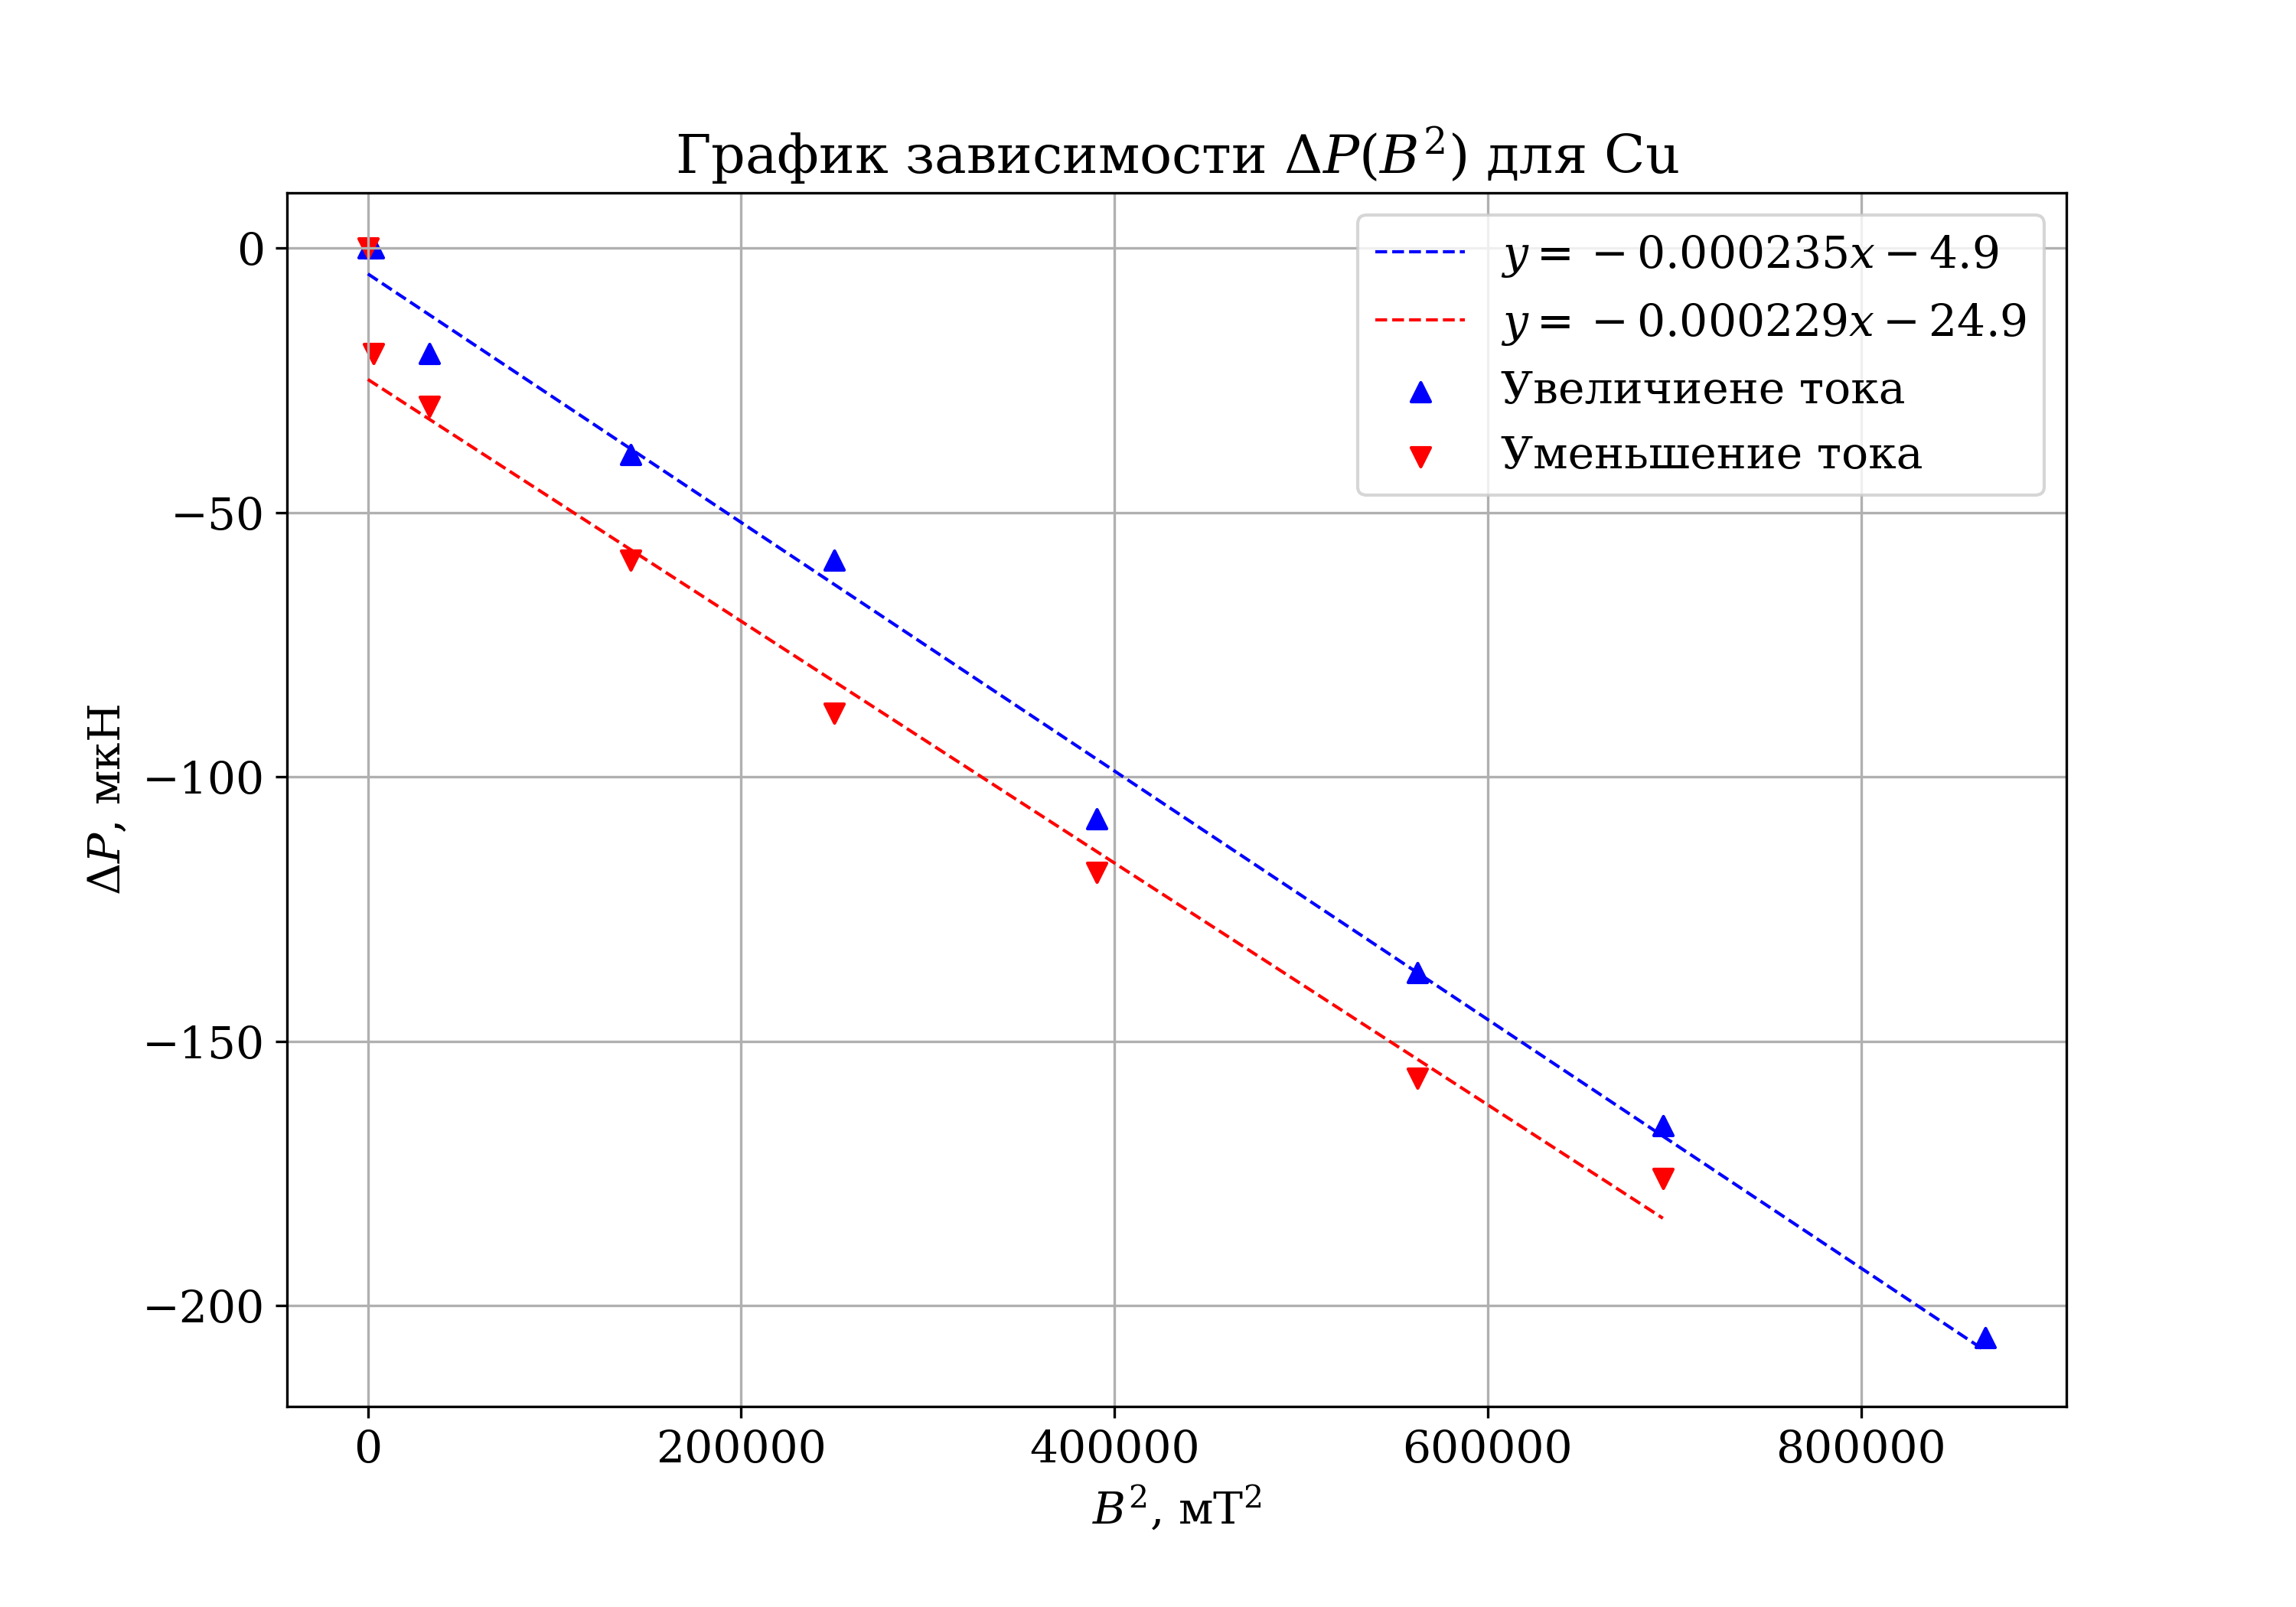
\includegraphics[width=0.85\linewidth]{plot_cu.png}
\caption{График для Cu}
\label{plot_cu}
\end{center}
\end{figure}

\begin{figure}[h!]
\begin{center}
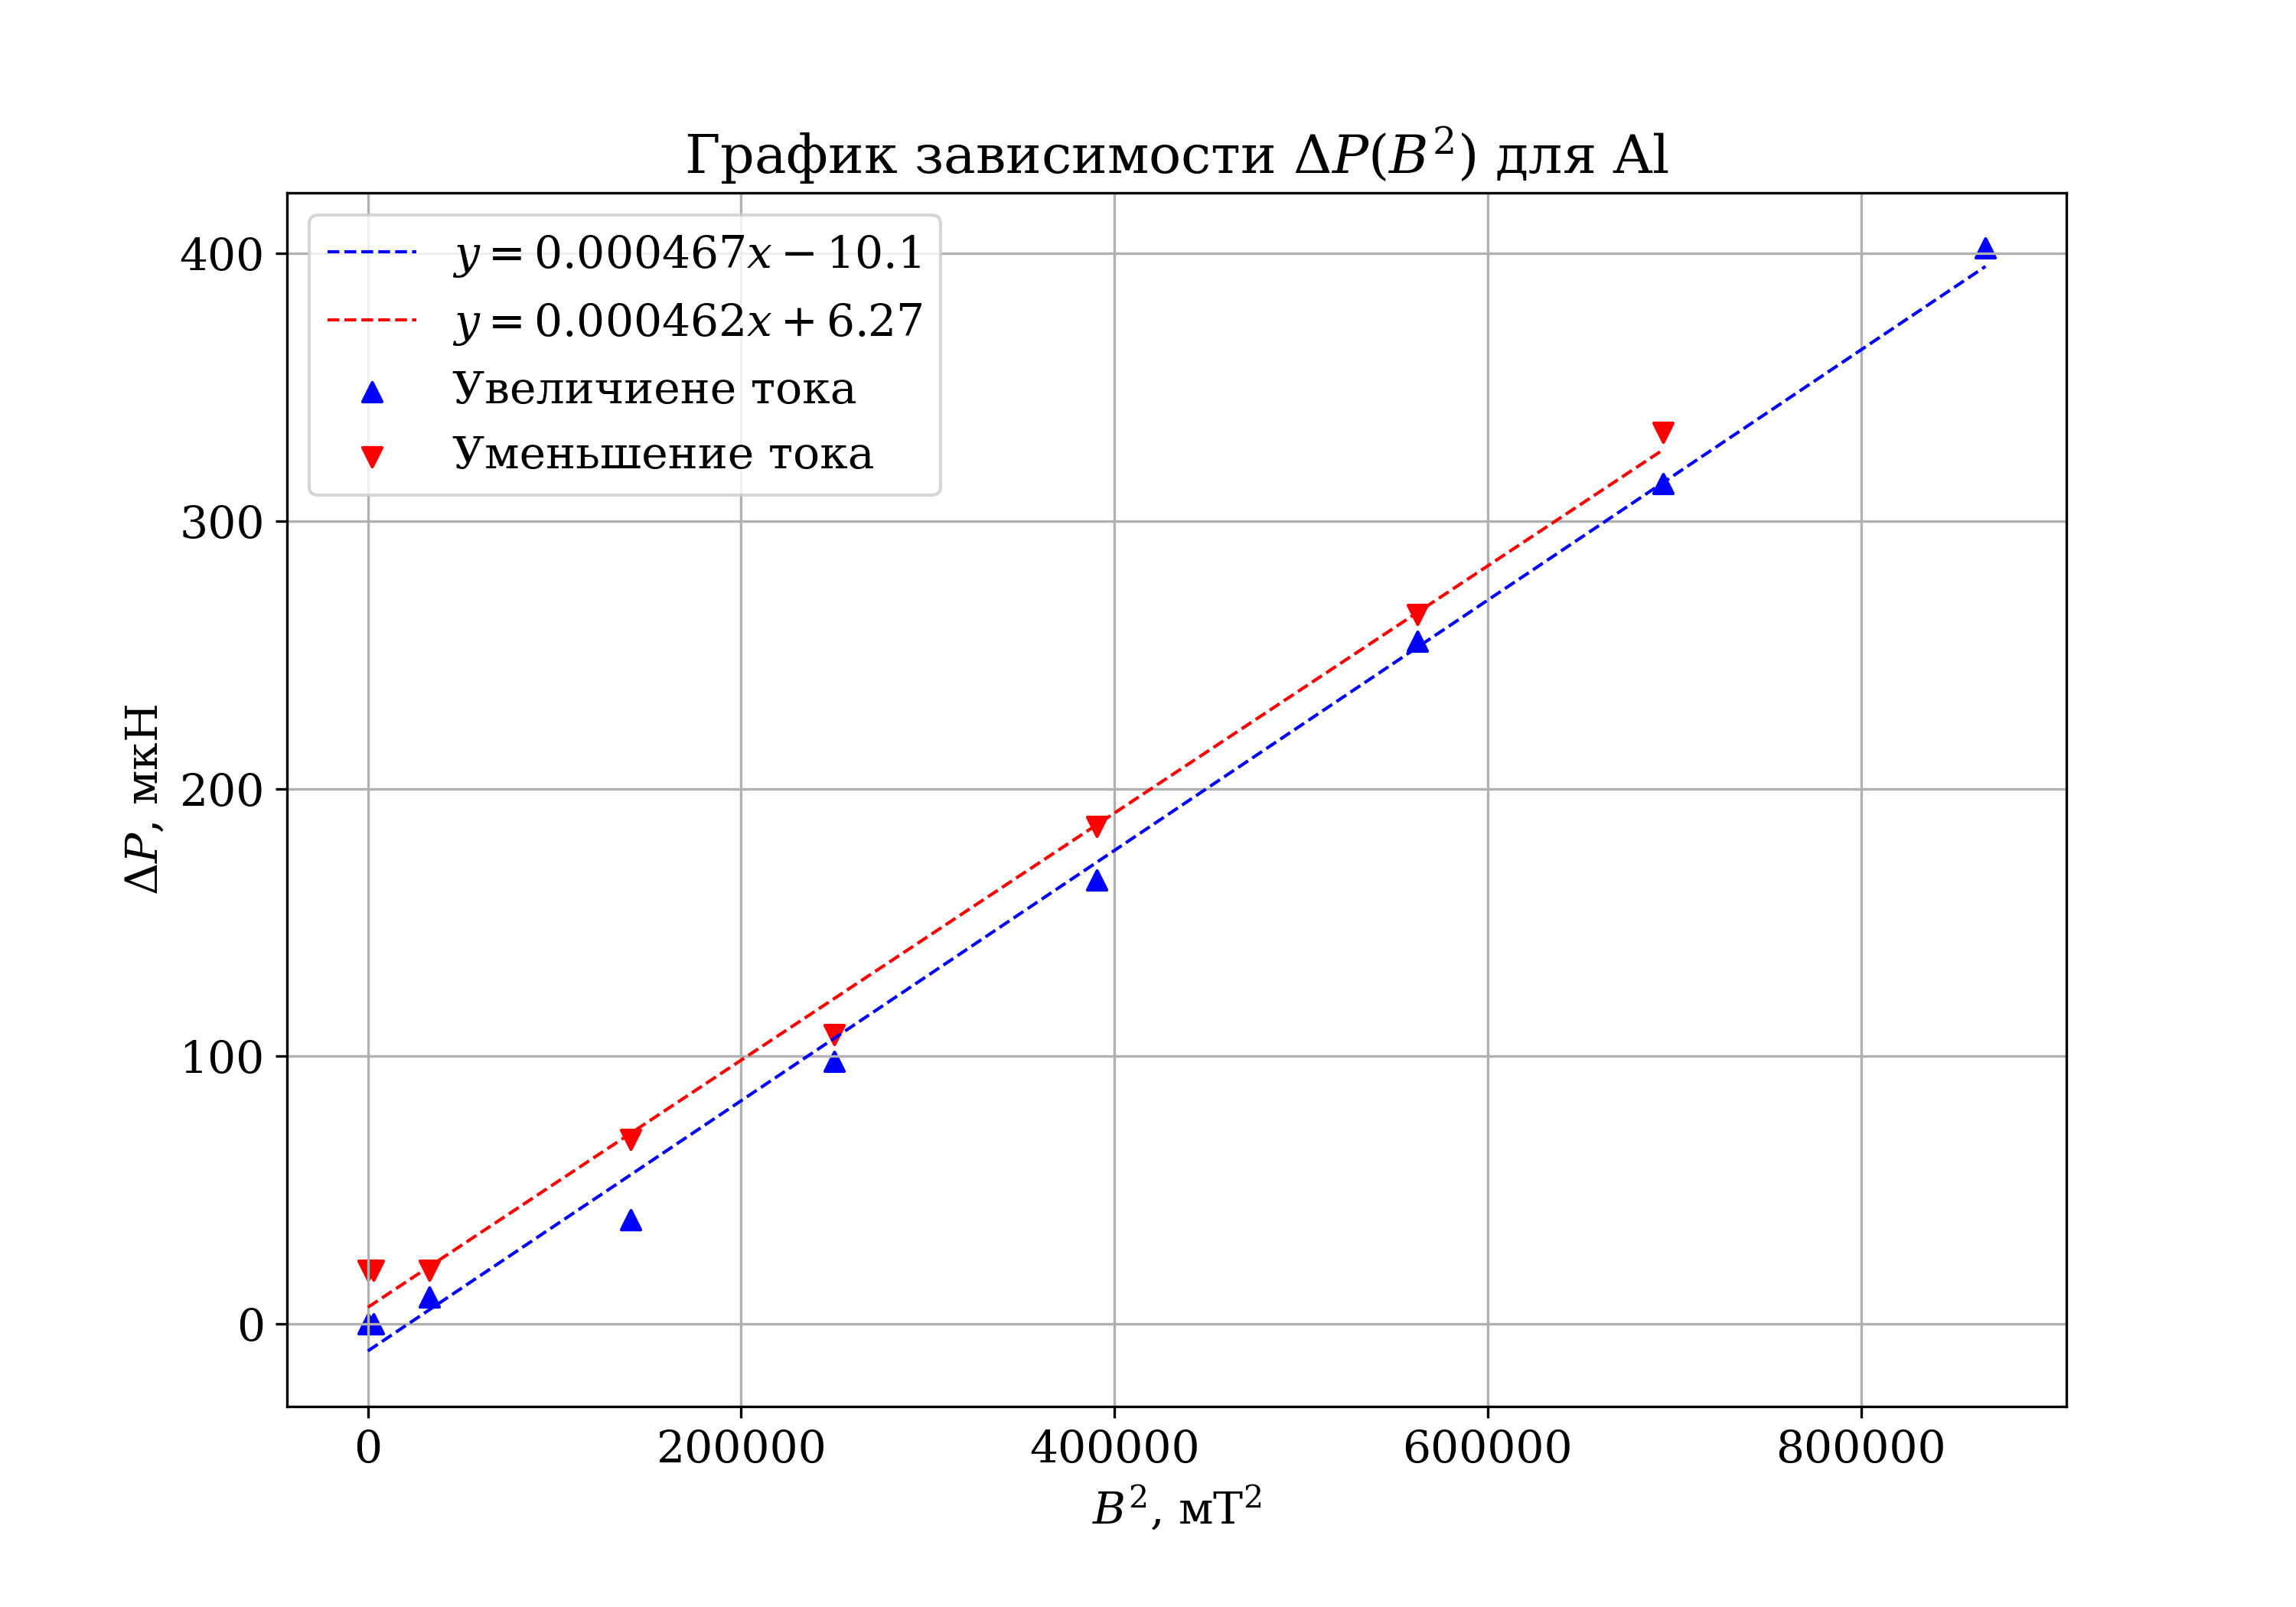
\includegraphics[width=0.8\linewidth]{plot_al.png}
\caption{График для Al}
\label{plot_al}
\end{center}
\end{figure}

\begin{figure}[h!]
\begin{center}
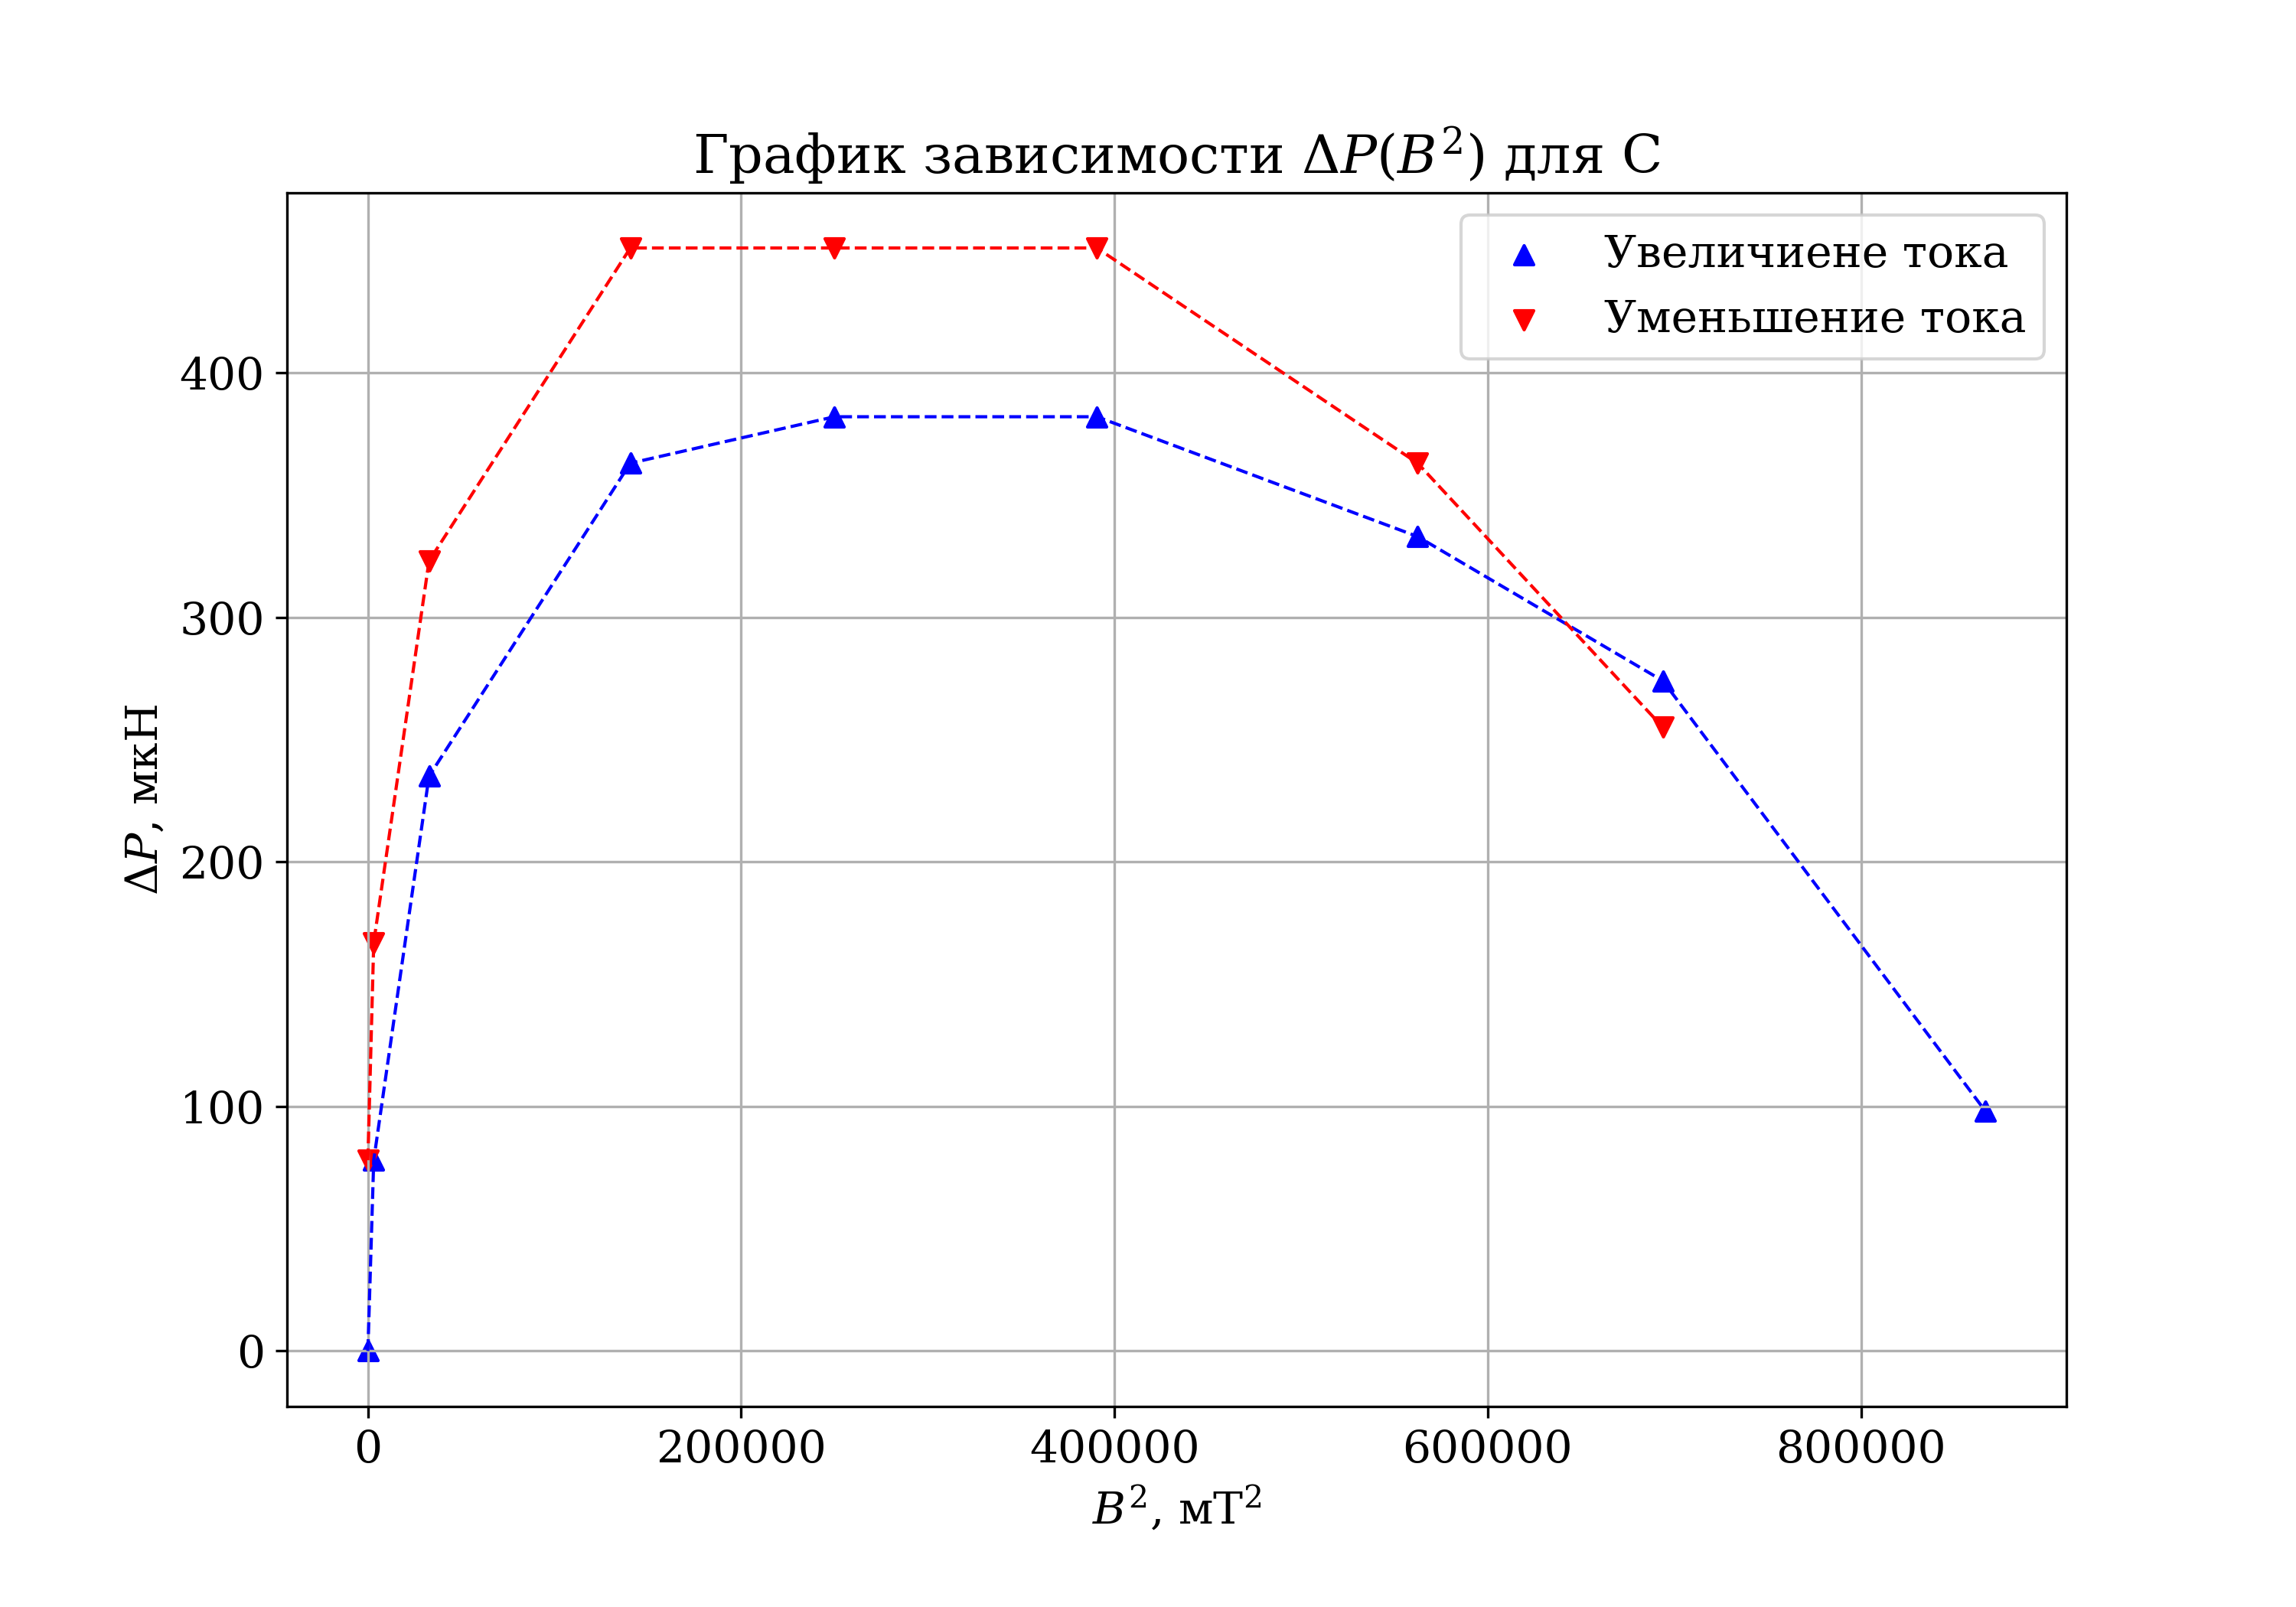
\includegraphics[width=0.8\linewidth]{plot_c.png}
\caption{График для C}
\label{plot_c}
\end{center}
\end{figure}

\item Получим значения $\chi$ и погрешности $\sigma_\chi$ пользуясь формулой:
\[ \Delta P = \frac{\chi s}{2 \mu_0} B^2 = \alpha B^2 \Rightarrow \chi = \frac{2 \alpha \mu_0}{s} \Rightarrow \chi_\text{уд} = \frac{2 \alpha \mu_0}{s \rho} ,\]
где $\alpha$ -- коэффициент наклона аппроксимирующей прямой рассчитанной пользуясь методом наименьших квадратов, $s$ -- площадь сечения образца $s = \pi d^2 / 4 = \pi / 4$ см$^2$. 

Для Cu получаем:

\[ \alpha_\blacktriangle = -(235 \pm 6) \cdot 10^{-6} \; \frac{\text{Н}}{\text{Тл}^2}, \]

\[ \alpha_\blacktriangledown =-(229 \pm 7) \cdot 10^{-6} \; \frac{\text{Н}}{\text{Тл}^2} \]

Берём среднее $\alpha_\textbf{Cu} = - (2.3 \pm 0.1) \cdot 10^{-4}$ Н/Тл$^2$, из чего получаем: 
\[\chi_\text{Cu} = - (8.2 \pm 0.4) \cdot 10^{-10} \;\frac{\text{м}^3}{\text{кг}}.\] 

Для Al получаем:

\[ \alpha_\blacktriangle = (467 \pm 9) \cdot 10^{-6} \; \frac{\text{Н}}{\text{Тл}^2}, \]

\[ \alpha_\blacktriangledown = (462 \pm 11) \cdot 10^{-6} \; \frac{\text{Н}}{\text{Тл}^2}. \]

Берём среднее $\alpha_\textbf{Al} = (4.6 \pm 0.2) \cdot 10^{-4}$ Н/Т$^2$, из чего получаем: 
\[\chi_\text{Al} =  (5.6 \pm 0.3) \cdot 10^{-9}\;\frac{\text{м}^3}{\text{кг}}.\] 

Для C график получился нелинейным, что может быть связано с тем, что в нем находятся примеси железа.

\end{enumerate}
\paragraph{Выводы:}
\begin{enumerate}
\itemsep0em
\item Мы провели исследование поведения диа- и парамагнетиков в магнитном поле и показали, что выполняются зависимости лежащие в основе метода Гюи.
\item нашли значения для удельной магнитной восприимчивости меди и алюминия

\[\chi_\text{Cu} = - (8.2 \pm 0.4) \cdot 10^{-10}\;\frac{\text{м}^3}{\text{кг}}, \;\;\; \chi_\text{Al} = (5.6 \pm 0.3) \cdot 10^{-9}\;\frac{\text{м}^3}{\text{кг}}.\]

Сравнивая с табличными значениями: 
\[\chi_\text{Cu, табл.} = - 8.6 \cdot 10^{-10}\;\frac{\text{м}^3}{\text{кг}}, \;\;\; \chi_\text{Al, табл.} = 6.1 \cdot 10^{-9}\;\frac{\text{м}^3}{\text{кг}}.\]

Видим, что измеренные значения достаточно близки к табличным
\item Увидели характер изменения $\Delta P(B^2)$ в графите. Предположительно, это происходит из-за примесей железа в графите.
\end{enumerate}
\end{document}